\chapter{Auswertung}

\section{Metriken zur Auswertung}

% auswertung hintergrundentfernung
\section{Hintergrundentfernung}

% auswertung randentfernung
\section{Randentfernung}

\section{Gesichtserkennung}
Die von OpenCV mitgelieferten Methoden zur Gesichtserkennung auf Bildern funktioniert grundsätzlich gut. Sie ist einfach anwendbar, hat eine vertretbare Laufzeit (der Algorithmus läuft nur einige Sekunden auf einer ganzen eingescannten Albumseite) und erkennt zumindest einen Großteil der Gesichter in den Fotos. \\
Um die Performanz der Classifier einzeln und in Kombination auszuwerten, wurden Wahrheitsmatrizen aufgestellt. Ausgewertet werden jeweils die korrekt erkannten Gesichter (True Positives (TP): positive - positive), die nicht erkannten Gesichter (False Negatives (FN): positive - negative) und die fälschlicherweise erkannten Gesichter (False Positives (FP): negative - positive). Korrekt nicht erkannte Gesichter (True Negatives (TN): negative - negative) gibt es in unserem Anwendungsfall nicht.\\
Tabellen \ref{tab:set1frontal} und \ref{tab:set2frontal} zeigen die Metriken in dem ersten und dem zweiten Datensatz wenn nur der frontal faces Classifier angewendet wird. Die daraus errechnete Genauigkeit \footnote{Formel für die Berechnung der Genauigkeit (\grqq Accuracy\grqq) ist: $\frac{TP + TN}{TP + FN + TN + FP}$, ($TN = 0$ in unserem Fall).} beträgt im ersten Datensatz 0.75 und im zweiten 0.59.\\
\begin{table}[h]
	\centering
	\begin{tabular}{l|lll}
		\hline
		& \multicolumn{3}{l}{Reference} \\ \hline
		\multirow{3}{*}{Prediction} &  & Positive & Negative \\
		& Positive & 270 & 1 \\
		& Negative & 88 & - \\ \hline 
	\end{tabular}
	\caption{Wahrheitsmatrix im ersten Datensatz, wenn nur der frontal-Classifier zum Einsatz kommt. Die Genauigkeit der Gesichtserkennung beträgt 0.75.}
	\label{tab:set1frontal}
\end{table}
\begin{table}[h]
	\centering
	\begin{tabular}{llll}
		\hline
		& \multicolumn{3}{l}{Reference} \\ \hline
		\multirow{3}{*}{Prediction} &  & Positive & Negative \\
		& Positive & 282 & 7 \\
		& Negative & 172 & - \\ \cline{2-4} 
	\end{tabular}
	\caption{Wahrheitsmatrix im zweiten Datensatz, wenn nur der frontal-Classifier zum Einsatz kommt. Die Genauigkeit der Gesichtserkennung beträgt 0.59.}
	\label{tab:set2frontal}
\end{table}
Wenn der zweite Classifier zur Erkennung von Profilen mit dazu genommen wird, erhöht sich die Anzahl der erkannten Gesichtern ein wenig. Das ist in Tabellen \ref{tab:set1frontalprofile} und \ref{tab:set2frontalprofile} zu sehen. Die Gesichter, die bereits von dem frontal-Classifier erkannt wurden, werden automatisch heraus gefiltert. Danach bleibt ein kleiner Mehrgewinn durch die Anwendung des profile-Classifiers übrig, die Performanz verbessert sich auf 0.76 und 0.65 jeweils.
\begin{table}[h]
	\centering
	\begin{tabular}{llll}
		\hline
		& \multicolumn{3}{l}{Reference} \\ \hline
		\multirow{3}{*}{Prediction} &  & Positive & Negative \\
		& Positive & 274 & 2 \\
		& Negative & 84 & - \\ \cline{2-4} 
	\end{tabular}
	\caption{Wahrheitsmatrix im ersten Datensatz, wenn frontal- und profile-Classifier kombiniert werden. Die Genauigkeit der Gesichtserkennung beträgt 0.76.}
	\label{tab:set1frontalprofile}
\end{table}
\begin{table}[h]
	\centering
	\begin{tabular}{llll}
		\hline
		& \multicolumn{3}{l}{Reference} \\ \hline
		\multirow{3}{*}{Prediction} &  & Positive & Negative \\
		& Positive & 301 & 8 \\
		& Negative & 153 & - \\ \cline{2-4} 
	\end{tabular}
	\caption{Wahrheitsmatrix im zweiten Datensatz, wenn frontal- und profile-Classifier kombiniert werden. Die Genauigkeit der Gesichtserkennung beträgt 0.65.}
	\label{tab:set2frontalprofile}
\end{table}

\subsubsection*{Festlegung der Ground Truth}
Die Referenz für die Auswertung der Gesichtserkennung festzulegen ist nicht trivial. Auf den alten Fotos sind aufgrund der schlechten Qualität der Aufnahmen viele Gesichter nicht tatsächlich zu erkennen. Vielmehr erschließt sich ein menschlicher Betrachter aus dem Kontext die Information, dass sich an gewissen Stellen ein Gesicht befinden muss. Das wurde bei der Festlegung der Ground Truth berücksichtigt. So wurden beispielsweise besonders kleine, verdeckte oder stark verschwommene Gesichter für die Berechnung der Metriken nicht berücksichtigt. Die Classifier haben außerdem Probleme, Gesichter zu erkennen, wenn starke Okklusionen auftreten, selbst wenn das Gesicht nur im Profil zu erkennen ist oder die Person eine Kopfbedeckung trägt. Diese wiederum wurden in die Gesamtsumme der Gesichter mit einberechnet. Im Folgenden werden exemplarisch einige Bilder gezeigt, die der Gesichtserkennungsalgorithmus nicht erkennen kann und die deswegen nicht in die Auswertung mit einbezogen wurden.\\
Bild \ref{fig:neg_ex1} zeigt ein kleines Mädchen, jedoch ist die Aufnahme sehr verschwommen. Jeder Mensch, der das Bild betrachtet, weiß, dass das Mädchen ein Gesicht haben muss. Wenn jedoch die Kontextinformationen entfernt werden würde, wäre es selbst für einen Menschen schwer, ein Gesicht zu identifizieren.\\
\begin{figure}[h]
	\centering
	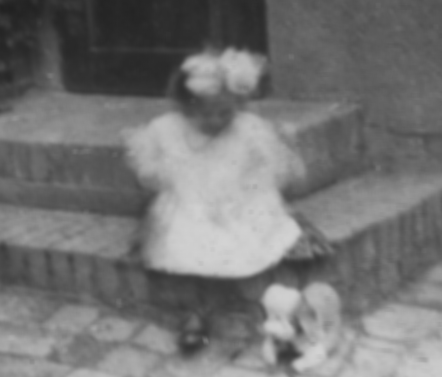
\includegraphics[width=0.75\linewidth]{images/examples_groundtruth/negative/04_1.png}
	\caption{Starke Bewegung im Bild verhindert, dass das Gesicht des Mädchens tatsächlich zu sehen ist, auch wenn menschliche Betrachter durchaus ihr Gesicht erkennen könnten.}
	\label{fig:neg_ex1}
\end{figure}
Auf Bild \ref{fig:neg_ex2} ist eine ähnliche Situationen zu sehen: alle abgebildeten Menschen haben Gesichter, jedoch sind sie objektiv nicht wirklich zu sehen. Sie sind relativ klein, was normalerweise für den Classifier kein Problem darstellt, aber eine schlechte Beleuchtung und geringer Kontrast tragen dazu bei, dass die Gesichter nicht erkannt werden.\\
\begin{figure}[h]
	\centering
	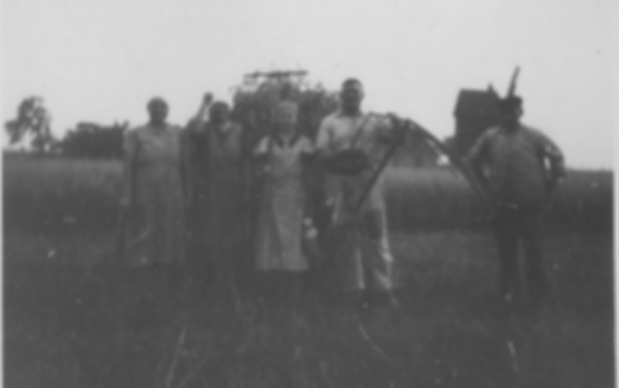
\includegraphics[width=0.75\linewidth]{images/examples_groundtruth/negative/29_2.png}
	\caption{Die Gesichtserkennung schlägt fehlt, wenn die Gesichter zu schlecht beleuchtet sind und/oder zu wenig Kontrast aufweisen. Auch, wenn normalerweise auch Gesichter in dieser Größe von dem Algorithmus problemlos erkannt werden.}
	\label{fig:neg_ex2}
\end{figure}
Um dennoch eine repräsentative Auswertung der Performanz der Gesichtserkennung zu gewährleisten, wurden viele nicht erkannte Gesichter mit in die Metriken einberechnet. Beispielsweise können die Classifier keine Gesichter mit Kopfbedeckungen erkennen. Ansonsten sind aber die Gesichter gut zu identifizieren, was in Bild \ref{fig:pos_ex1} zu sehen ist.\\
\begin{figure}[h]
	\centering
	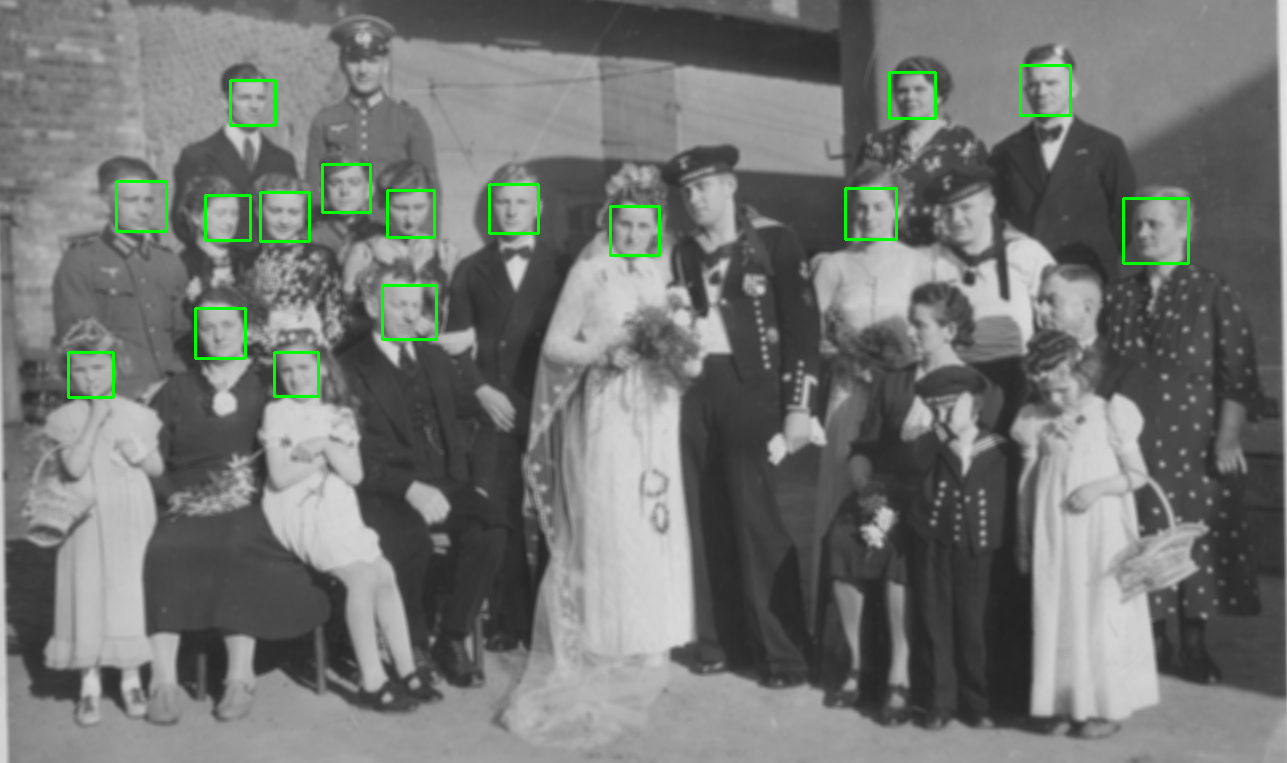
\includegraphics[width=0.75\linewidth]{images/examples_groundtruth/positive/32_3.png}
	\caption{Kein Classifier erkennt Gesichter mit Hüten, auch wenn sie nur einen kleinen Teil vom Gesicht verdecken. Alle anderen Gesichter werden problemlos identifiziert.}
	\label{fig:pos_ex1}
\end{figure}
Bild \ref{fig:pos_ex2} zeigt einen problematischen Grenzfall aus dem zweiten Datensatz. In diesem Bild wurden insgesamt drei Gesichter erkannt (zwei vom frontal-Classifier (grün) und eins vom profile-Classifier (rot)). Da alle Gesichter in etwa die gleiche Größe und Schärfe haben, sollte angenommen werden, dass auch die restlichen Personen erkannt werden. Es ist nicht ersichtlich, warum auf diesem Bild beide Classifier keine weiteren Gesichter erkennen. Von daher fließen alle Gesichter auf diesem Foto mit in die Bewertung ein und erhöhen die Anzahl der False Negatives enorm. Besonders im zweiten Datensatz kommen solche Fälle häufiger vor, was die schlechte Performanz des Algorithmus' im Vergleich zum ersten Datensatz erklärt.
\begin{figure}[h]
	\centering
	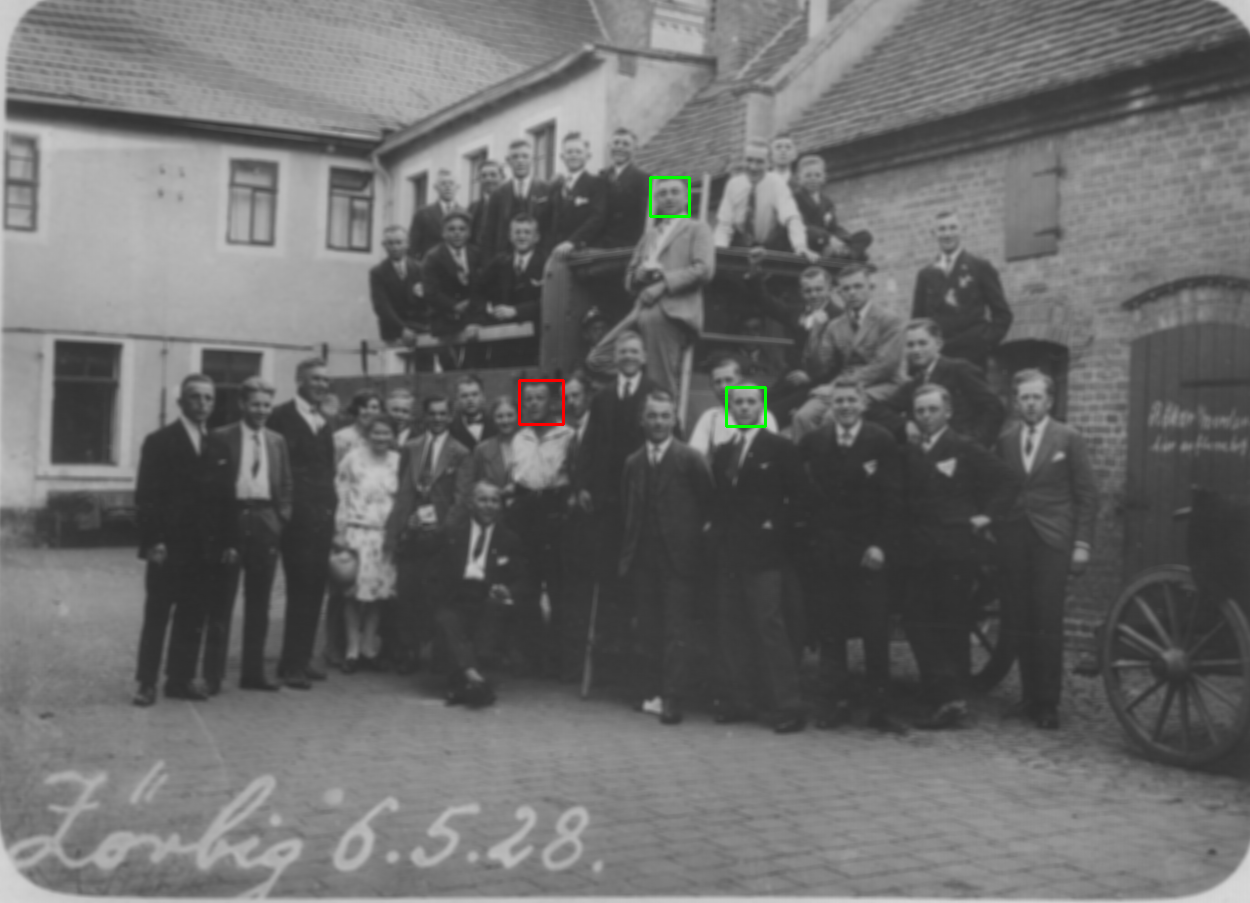
\includegraphics[width=0.75\linewidth]{images/examples_groundtruth/positive/16_1.png}
	\caption{In diesem Gruppenfoto werden nur wenige Gesichter erkannt, obwohl sie alle ähnlich aussehen. Das verschlechtert die Kennwerte für die Genauigkeit besonders im zweiten Datensatz stark.}
	\label{fig:pos_ex2}
\end{figure}